\documentclass[
12pt, % Main document font size
a4paper
%, % Paper type, use 'letterpaper' for US Letter paper
%oneside, % One page layout (no page indentation)
%twoside, % Two page layout (page indentation for binding and different headers)
%headinclude,footinclude, % Extra spacing for the header and footer
%BCOR5mm, % Binding correction
]{report}

\usepackage[font=small,labelfont=bf,justification=raggedright,format=hang,singlelinecheck=off,textfont=it]{caption}
%\usepackage{subcaption}
\usepackage{indentfirst}
\usepackage{longtable}
\usepackage{tabu}
\usepackage{titlepic}
\usepackage{geometry}
\geometry{margin=1in,top=1.5in,bottom=1.5in}
\usepackage{mathtools}
\usepackage{polski}
\usepackage[utf8]{inputenc}
\usepackage{booktabs}
\usepackage[T1]{fontenc}
\usepackage{lmodern}
\usepackage{fancyhdr}
\pagestyle{fancy}
\pagestyle{headings}
\usepackage{float}
\usepackage{graphicx}
\usepackage{listings}
\usepackage{enumitem}
\usepackage{titlesec}
\usepackage{pdfpages}
\usepackage{wallpaper}
%\usepackage{cleveref}
\usepackage{afterpage}

\usepackage{hyperref}
\hypersetup{
    colorlinks,
    citecolor=black,
    filecolor=black,
    linkcolor=black,
    urlcolor=black
}

\usepackage{cleveref}

\newcommand\blankpage{%
    \null
%	\ClearWallPaper
    \thispagestyle{empty}%
    \addtocounter{page}{-1}%
    \newpage
%	\ULCornerWallPaper{1}{head}
}

%\captionsetup{}

%\usepackage{showframe}


\newcounter{magicrownumbers}
\newcommand\rownumber{\stepcounter{magicrownumbers}\arabic{magicrownumbers}}

%variables
\newcommand{\shopname}{SHOP NAME}
\newcommand{\companyname}{COMPANY NAME}
\newcommand{\regon}{REGON}
\newcommand{\nip}{NIP}
\newcommand{\httpaddr}{SITE ADDRESS}
\newcommand{\address}{ADDRESS}
\newcommand{\mail}{MAIL ADDRESS}
\newcommand{\phone}{PHONE NUMBER}
\newcommand{\currency}{CURRENCY}

\setlistdepth{9}
\graphicspath{ {images/} }

\title{Dokumentacja modułu}
\author{RobCo sp. z o.o.}
%\titlepic{
\includegraphics[width=128px]{logo.png}}

%definitions
\newif\ifpersonal
\personaltrue % comment out to hide answers

%styling
\titlespacing*{\subparagraph}{1em}{0pt}{0pt}
\titleformat{\subparagraph}[runin]
{\normalfont\normalsize}{\thesubparagraph}{1em}{}

%\ULCornerWallPaper{1}{head}
%\LLCornerWallPaper{1}{foot}

\begin{document}			


	%strona tytulowa
	\begin{titlepage}
	\clearpage\maketitle
	\thispagestyle{empty}
\end{titlepage}


	\afterpage{\blankpage}
	
	%spis tresci
	% Set the depth of the table of contents to show sections and subsections only
%\setcounter{tocdepth}{2} 
\newpage 
\tableofcontents % Print the table of contents
\newpage


	%pojecia
	\chapter{Wstęp}
        \section{Pojęcia}
		\section*{Definicje}
\addcontentsline{toc}{section}{Pojęcia}
	Pojęcia z jakimi należy się zaznajomić:
	\begin{description}
	
		\item[\textbf{Pojęcie}] - opis

	\end{description}

		\section{Założenia projektu} 
		\part{Założenia projektu} 

		
    \chapter{Architektura}
     

        \section{Platforma sprzętowa}
         
\part{Platforma sprzętowa}
    
    \input{raspberry_pi.tex}
    \input{atomic_pi.tex}
    \input{banana_pi.tex}
    \input{obudowa.tex}
    

            \subsection{Raspberry Pi}
            \input{raspberry_pi.tex}
            \subsection{Atomic Pi}
            \input{atomic_pi.tex}
            \subsection{Banana Pi}
            \input{banana_pi.tex}
            \subsection{Obudowa}
            \input{obudowa.tex}
        \section{System} 
            Linux

        \section{Aplikacja} 
        \part{Aplikacja} 

            \subsection{Biblioteka bazowa}
             

                \subsubsection{Obiekt}
                 

                    \paragraph{Fabryka}
                     

                    \paragraph{Terminal}
                     

                    \paragraph{Powłoka}
                     

                    \paragraph{Urządzenie}
                     

                        \subparagraph{ADC}
                         

                        \subparagraph{DAC}
                         

                        \subparagraph{CAN}
                         

            \subsection{Moduły}
             

                \subsubsection{Powłoka komend}
                 

                \subsubsection{Powłoka Python}
                 

                \subsubsection{Powłoka Lua}
                 

                \subsubsection{Terminal strumieniowy}
                 

                \subsubsection{Sterownik ADS1256}
                 

                \subsubsection{Sterownik DAC8532}
                 


	\chapter{Rozszerzenia}
	 

        \section{Przetwornik analogowo cyfrowy}
         

        \section{Przetwornik cyfrowo analogowy}
         

        \section{Szyna CAN}
         

        \section{Tranzystor IGBT}
         

            \subsection{Bezpośrednie podłączenie}
             

            \subsection{Podłączenie przez przetwornik}
             

	\chapter{Eksploatacja}
	 

        \section{Instalacja}
         

        \section{Konfiguracja}
         

            \subsection{Tryby pracy}
             

                \subsubsection{Samodzielny}
                 

                \subsubsection{Sieciowy}
                 

            \subsection{Programy wsadowe}
             

        \section{Integracja}
         

            \subsection{InfluxDB}
             

            \subsection{Grafana}
             

            \subsection{Graphite}
             

            \subsection{Legacy}
             

    \chapter{Dodatki}
        \section{Licencja}
         

        \section{Karta Gwarancyjna}
         

						
	\chapter{Elementy}
		\section{Obraz} 

		\begin{figure}[H]
			\centering
			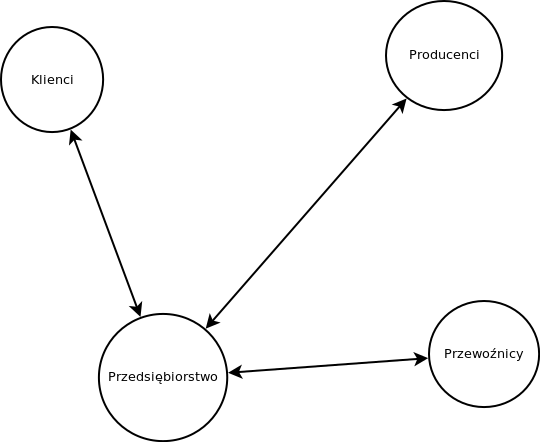
\includegraphics[scale=0.45]{groups}
			\caption{Przepływ informacji między grupami ludzi}
			\label{groups}
		\end{figure} 	

		\section{Wypunktowanie}
	\begin{itemize}	
		\item Mocne strony
			\begin{itemize}
				\item duże doświadczenie w pracy w handlu
				\item wysoka jakość towarów i usług
				\item bardzo dobrze przygotowany system komputerowy
				\item przejrzysty interface sklepu internetowego
				\item niskie koszty prowadzenia działalności
				\item dobra znajomość rynku
				\item sklep międzynarodowy
			\end{itemize}
			
		\item Słabe strony
			\begin{itemize}
				\item niski kapitał własny
				\item brak doświadczenia w prowadzeniu własnej działalności gospodarczej
				\item brak dodatkowych pracowników na początku prowadzenia działalności
				\item brak doświadczenia w handlu międzynarodowym
			\end{itemize}
			
		\item Szanse
			\begin{itemize}
				\item rosnąca zamożność społeczeństwa
				\item łatwa dostępność do sklepu internetowego
				\item rosnące zainteresowanie e-handlem
				\item wprowadzenie kompleksowej umowy gospodarczo-handlowej CETA
			\end{itemize}
			
		\item Zagrożenia
			\begin{itemize}
				\item duża konkurencja
				\item wysokie koszty zakupu sprzętu komputerowego
				\item zaniżanie cen produktów przez konkurencje
				\item niestabilność prawa gospodarczego
				\item brak wystarczającej ilości producentów chętnych współpracować ze sklepem
				\item możliwe rosnące ceny surowców
			\end{itemize}
	\end{itemize}

        \section{Tabela}

		\begin{table}[H]
			\centering
			\begin{tabular}{|l|l|l|l|}
			\hline
																															& Miasto   & Wieś     & Razem    \\ \hline
			\begin{tabular}[c]{@{}l@{}}Liczba gospodarstw \\ domowych\end{tabular}               & 9400000  & 4700000  & 14100000 \\ \hline
			\begin{tabular}[c]{@{}l@{}}Liczba osób w gospodarstwach \\ domowych\end{tabular}     & 22842000 & 15322000 & 38164000 \\ \hline
			\begin{tabular}[c]{@{}l@{}}Średnia liczba osób\\ na gospodarstwo domowe\end{tabular} & 2.43     & 3.26     & 2.71     \\ \hline
			\end{tabular}
			\caption{Tabela dane dotyczące zamieszkania w Polsce}
			\label{avg_home_pl}
		\end{table}

		
		\begin{table}[H]
		\centering
		\begin{tabular}{|l|l|l|l|}
		\hline
					& Polska \textless-\textgreater Polska [zł] & Kanada \textless-\textgreater Kanada [zł] & Polska \textless-\textgreater Kanada [zł] \\ \hline
		Komody 	& 69                                 & 414                                & 960                                \\ \hline
		Fotele 	& 51                                 & 408                                & 960                                \\ \hline
		Sofy   	& 480                                & 1225                               & 1606                               \\ \hline
		Stoły  	& 94                                 & 1137                               & 960                                \\ \hline
		Łóżka  	& 321                               	& 1167                               & 1200                               \\ \hline
		\end{tabular}
		\caption{Średnia cena transportu wybranych grup produktów}
		\label{avg_grp_shp_price}
		\end{table}
		

        \section{Paragrafy}

    \subsection{Opis}
        \par W pierwszym roku prowadzenia działalności mojej firmy będę jej jedynym pracownikiem. Będę odpowiedzialna za pozyskiwanie producentów, których produkty będą prezentowane na stronie, obsługą klientów, logistyką oraz będę się zajmować innymi działaniami niezbędnymi do prowadzenia sklepu internetowego. W trakcie rozwoju firmy planuję zatrudnienie pracowników, którzy przejmą ode mnie część obowiązków. Wprowadzając awanse pionowe, oznaczające pięcie się "w górę" na coraz to wyższe stanowiska w firmie, w drugim roku handlowiec awansuje na stanowisko starszego handlowca, robiąc tym samym lukę, co pozwala na zatrudnienie nowej osoby na stanowisko handlowca. Powielając ten schemat w trzecim roku, starszy handlowiec awansuje na stanowisko kierownika; handlowiec zostanie starszym handlowcem. W ten sposób można zatrudnić kolejną osobę, która zapełni lukę w hierarchii organizacyjnej przedsiębiorstwa. 
			 

				
    \subsubsection{Wynagrodzenia}
        \par Przez "wynagrodzenie" rozumiemy ekwiwalent należny za pracę pracownika na rzecz pracodawcy w ramach stosunku pracy. W trakcie rozwoju firmy mam zamiar zatrudniać pracowników na postawie umowy o pracę. Wynagrodzenie początkowe jakie będzie otrzymywał pracownik, to wynagrodzenie minimalne, które zostało ujęte w kodeksie pracy. Na dzień dzisiejszy wynosi ono 2000 zł. brutto. Po otrzymanym awansie, pracownik będzie otrzymywał coraz wyższe wynagrodzenie adekwatne do zajmowanego stanowiska. Można przyjąć, iż będą to podwyżki na poziomie 20-30 \%.
			
        \par Jak powszechnie wiadomo wynagrodzenie pracownika pełni nie tylko funkcję czysto dochodową. Również bardzo ważną jest tu funkcja motywacyjna- im większy wpływ na swoją płacę ma pracownik, tym większą ma motywację do pracy. Dlatego bardzo ważne jest wprowadzenie systemu premii, nagród itp.. W moim przypadku może być to premia związana ze wzrostem sprzedaży, sumienności wykonywanych obowiązków, czy też zaangażowania w rozwój sklepu.

        
\end{document}
